\documentclass{article}
\usepackage{iclr2027_conference}
\usepackage{times}
\usepackage{amsmath,amssymb,amsfonts}
\usepackage{booktabs}
\usepackage{graphicx}
\usepackage{xcolor}
\usepackage{multirow}
\usepackage[hidelinks]{hyperref}

% NOTE: compiled against an ICLR-2025-derived style file renamed to
% iclr2027_conference.sty. Replace it with the official iclr2027_conference.sty
% when ICLR releases the 2027 template; the preamble should not need changes.

% Citation placeholder: the references section is intentionally omitted for now.
\newcommand{\refadd}[1]{\textcolor{blue}{[REF: #1]}}
% Pending-result placeholder.
\newcommand{\pending}[1]{\textcolor{red}{[TODO: #1]}}

% 投稿版保持下面一行注释状态（页眉显示 Under review）；-camera-ready 时取消注释
% \iclrfinalcopy

\title{Learning Where to Read: Adaptive Node-Reveal Policies for\\ Budget-Limited Graph Classification}

\author{Anonymous authors\\ Paper under double-blind review}

\newcommand{\reveal}{\textsc{reveal}}

\begin{document}

\maketitle

\begin{abstract}
Graph classifiers almost universally assume that the full graph is available at prediction time, yet on large graphs the discriminative evidence is often concentrated in a small region, and inspecting nodes and edges carries real cost. We study \emph{budget-limited active graph reading}: starting from a single seed node, an agent repeatedly selects frontier nodes to reveal under a fixed node budget, and then classifies the revealed subgraph. We contribute a leak-proof evaluation protocol in which unvisited content is provably never used, and frontier edge features are free to query before a node is revealed; a two-stage learner that distills heuristic teachers into a reveal policy by behavior cloning and then fine-tunes it with reinforcement learning against a frozen, full-graph classifier; and an evidence reader that accumulates revealed evidence in a recurrent state decoupled from the reveal policy. On COLLAB, all fixed strategies collapse to the majority-class rate ($\approx 0.16$), while the learned policy reaches $0.52$--$0.56$ on the test split at $10$--$20\%$ budgets, recovering up to $85\%$ of the full-graph test accuracy. On CIFAR10 superpixels, reinforcement fine-tuning outperforms the best fixed strategy by up to $11.3$ percentage points. Ablations show that recurrent evidence accumulation is the largest contributor. Gains narrow at very small budgets, on PPA the learned policy does not yet surpass the best fixed strategy, and some classes remain unsolved, bounding the current scope of the approach.
\end{abstract}

\section{Introduction}
\label{sec:intro}

Graph classification drives applications from security provenance analysis to molecular screening, and the dominant paradigm trains and evaluates on fully observed graphs. The assumption is convenient for benchmarks but unnatural for large graphs, where inspecting every node and edge is expensive or slow, and for noisy graphs, where most of the content is irrelevant to the label. In provenance graphs, program-dependence graphs, and large interaction graphs, the evidence that determines the label often lives in a small subgraph \refadd{evidence-concentration-in-graphs}.

If only a fraction of a graph can be inspected, the order of inspection matters. A breadth-first sweep wastes budget on irrelevant neighborhoods; a degree-greedy sweep ignores the task. Deciding \emph{where to read next} is a sequential decision problem: each revealed node changes what is visible at the frontier and what is worth revealing later. Practitioners of large language-model agents face the same constraint when they must decide what to retrieve next under a context budget, and solve it with learned, task-aware policies \refadd{llm-agent-context}.

Prior work offers partial answers, but each stops short of this setting. Graph-pooling methods such as SAGPool select informative subgraphs, yet they score nodes on the \emph{full} graph, assuming precisely the inspection we want to budget \refadd{sagpool,graph-pooling}. Subgraph sampling provides structure-only, task-agnostic views \refadd{subgraph-sampling}. Graph-explanation methods such as SubgraphX rationalize a trained full-graph model \emph{after} the graph has been read \refadd{subgraphx,graph-explainability}. Active learning on graphs budgets labels, and active feature acquisition budgets attributes, but neither budgets \emph{sequential structural observation} starting from a seed \refadd{active-learning-graphs,feature-acquisition}. What is missing is a protocol that makes partial graph observation leak-proof and reproducible, together with evidence that a learned policy outperforms fixed strategies under a matched budget.

We address both gaps. We formalize budget-limited active graph reading with a visibility protocol in three tiers: the frontier's existence (T0) and frontier edge features (T1) are visible before reveal at zero cost, while any property of unvisited nodes (T2) is forbidden to the predictor; deterministic seeds and a single-schema evaluation make results reproducible, and unit tests enforce that identical revealed sets yield identical predictions. We then train reveal policies in two stages: behavior cloning (BC) distills successful trajectories from heuristic teachers, and reinforcement learning (RL) fine-tunes the policy with an asymmetric reward computed by a frozen full-graph classifier. A separate evidence reader accumulates what has been read in a recurrent state, keeping the decision of \emph{where to read} decoupled from the decision of \emph{what has been learned}.

Our contributions are:
\begin{itemize}
  \item \textbf{Protocol.} A leak-proof benchmark for budget-limited graph reading on three datasets (OGBG-PPA, CIFAR10 superpixels, COLLAB), with matched budgets of $5$--$20\%$ of nodes, deterministic seeds, and invariant-based leakage tests.
  \item \textbf{Method.} A two-stage BC-then-RL learner with an asymmetric reward against a frozen classifier, and a recurrent evidence reader that separates evidence accumulation from node selection.
  \item \textbf{Findings.} On COLLAB, every fixed strategy, including SAGPool, collapses to the majority-class rate, while the learned policy recovers $79$--$85\%$ of full-graph test accuracy at $10$--$20\%$ budgets. On CIFAR10 superpixels, RL beats the best fixed strategy by up to $11.3$ points and BC by up to $14.3$ points at $15\%$ budget. Ablations attribute the largest share of accuracy to recurrent evidence accumulation.
\end{itemize}

\section{Related work}
\label{sec:related}

\paragraph{Graph classification and pooling.}
Message-passing classifiers consume the whole graph, and pooling methods sparsify it by scoring nodes with task-aware attention on the full graph; SAGPool is the representative we compare against \refadd{graph-pooling,sagpool}. Because these methods score nodes after the full graph is available, they answer a different question: which nodes \emph{matter}, not which nodes to inspect \emph{next} under a budget. We adapt SAGPool as a static-selection baseline under matched budgets and find that it, too, requires full-graph context to work well.

\paragraph{Subgraph sampling and task-agnostic selection.}
Sampling-based views (random walks, neighborhood expansion, graph cores) produce subgraphs without consulting the task \refadd{subgraph-sampling}. They are cheap and sequential-friendly, which is why several of them serve as our fixed baselines; their failure on COLLAB (Section~\ref{sec:results}) shows that task-agnostic selection cannot escape majority-class collapse there.

\paragraph{Graph explainability.}
Explanation methods such as SubgraphX identify rationales for a model's prediction on an already-observed graph \refadd{subgraphx,graph-explainability}. Our setting inverts the direction: evidence must be acquired before prediction. We still use explanation-style scoring as a teacher and as a static baseline, but the learned policy must act under partial observation, where such scores are unavailable by construction.

\paragraph{Active learning and feature acquisition on graphs.}
Active learning on graphs budgets \emph{labels} for training \refadd{active-learning-graphs}; active feature acquisition budgets \emph{attributes}, typically chosen in one shot or per column \refadd{feature-acquisition}. Our budget is on sequential structural observation at test time, which changes both the action space and the leakage risks. Evidential and POMDP-style readers accumulate observations for prediction \refadd{evidential-pomdp}; our evidence reader follows this line but is trained decoupled from the selection policy and evaluated under a strict no-leak protocol.

\section{Problem setup}
\label{sec:setup}

Let $G=(V,E)$ be a graph with label $y$, and let $R_t \subseteq V$ denote the revealed set after $t$ steps, $|R_0|=1$. The initial state is a single seed node drawn by a deterministic formula from the graph index and a seed counter, together with its incident edge list: the agent knows which neighbors exist (T0) and can query the features of edges from revealed to unrevealed nodes (T1) at zero budget cost, but no attribute or structure of unvisited nodes (T2). At each step $t<B$, the policy chooses a frontier node $v \in \partial R_t$ and the environment applies $\reveal(v)$: $v$ joins $R_t$, and the features of edges from $v$ to already-revealed nodes become visible. After $B$ steps the classifier predicts $y$ from the revealed subgraph. The budget $B$ is reported as a fraction of $|V|$; all comparisons in this paper are at matched budget ratios, averaged over four deterministic seeds.

Two invariants make the protocol leak-proof and are enforced by unit tests: (i)~the prediction is a function of the revealed set only, so the same revealed set at two budgets yields the same prediction, and (ii)~no embedding of an unrevealed frontier node enters the predictive path; we verify this by poisoning frontier embeddings with random noise and asserting that the prediction does not change. The T1 tier, free frontier edge features before reveal, is the deliberate distinction from protocols that hide all unrevealed content: it is the information a real inspector could obtain by looking at the boundary of what is already open.

\section{Method}
\label{sec:method}

\subsection{Overview}
Training proceeds in two stages. First, heuristic teachers generate reading trajectories, filtered to successful ones, and the reader is distilled by behavior cloning. Second, the policy is fine-tuned with reinforcement learning using a reward computed by a frozen full-graph classifier, which also serves as the reference head during evaluation. The classifier itself is trained once on full graphs and kept fixed throughout.

\subsection{Reader architectures}
The \textbf{base reader} encodes the revealed subgraph with a GIN encoder that integrates frontier edge features (T1), scores every frontier node with an MLP head, and reveals the argmax. Policy-side features, the remaining budget ratio and frontier summary statistics, are concatenated only into the selection scores and never reach the predictive path, as required by the invariants of Section~\ref{sec:setup}.

The \textbf{evidence reader} adds a recurrent evidence accumulator. After each reveal, the embeddings of revealed nodes are pooled into an evidence state $z_t$ by an LSTM over the reading trajectory; the final prediction uses the evidence head on $z$, and the selection head is unchanged. Two design choices follow from failures of an earlier, heavier variant. First, the accumulator only reads embeddings of \emph{revealed} nodes: a two-layer encoder cannot let evidence from distant revealed nodes interact within one forward pass, and the recurrence supplies that interaction across steps. Second, selection and prediction are separate heads on a shared encoder: routing the recurrent state into the pointer was the main cause of non-convergence in the earlier variant, whose parameter count was $4.6\times$ the base reader's while its per-step supervision, one action bit, stayed the same. The evidence reader instead has roughly the base reader's selection cost plus a small recurrent head.

\subsection{Teacher trajectories and behavior cloning}
Teachers generate reading trajectories by gradient saliency, information gain, and structural heuristics, as well as hybrid combinations \refadd{teacher-details-SI}. Trajectories are scored by the frozen classifier's accuracy on the finally revealed subgraph, filtered to successful ones, and balanced across classes. BC then maximizes the likelihood of the teacher's action at each step.

\subsection{Reinforcement fine-tuning}
BC inherits the teachers' biases and plateaus well below the full-graph classifier. RL fine-tuning treats reveal steps as actions with reward from the frozen classifier: success yields a large bonus, and a shaped per-step term credits trajectories that make the revealed subgraph \emph{more} informative, which mitigates the sparsity that stalls binary-reward REINFORCE when only $\sim$$12\%$ of training trajectories succeed. We call this the \emph{asymmetric} reward and ablate the reward family in the supplement \refadd{reward-ablation-SI}. Advantages are computed per trajectory with optional normalization; on filtered training data, training time halves without loss of test accuracy.

\section{Experiments}
\label{sec:results}

\subsection{Setup}
\label{sec:setup-exp}
We evaluate on three graph-classification benchmarks chosen for large per-graph scale: \textbf{OGBG-PPA} \refadd{ogbg}, \textbf{CIFAR10 superpixels} \refadd{lrgb}, and \textbf{COLLAB} \refadd{tudataset}. Budget ratios are $5/10/15\%$ for PPA and CIFAR10, and $10/15/20\%$ for COLLAB. Every number is the mean over four deterministic seeds. Fixed baselines are Random, BFS, Max-Frontier-Degree, and Random-Walk reveal, plus SAGPool adapted as a static selector; the frozen full-graph classifier provides the upper bound for each dataset, and its accuracy on revealed subgraphs is reported as a reference head. All results use the unified evaluation schema. For datasets with a validation split (PPA, COLLAB), every table cell reports validation\,/\,test; CIFAR10 has no validation split and reports test.

\begin{table}[t]
\centering
\caption{CIFAR10 superpixels, test accuracy (\%), mean of 4 seeds. Budget is the fraction of nodes revealed. The reference head is the frozen full-graph classifier evaluated on the RL-revealed subgraphs. BC denotes the main behavior-cloned reader configuration; the evidence-reader BC variants are ablated separately in Table~\ref{tab:ablation}.}
\label{tab:cifar10}
\footnotesize
\setlength{\tabcolsep}{4pt}
\begin{tabular}{lcccccccc}
\toprule
Budget & Random & BFS & Max-Front.-Deg. & Rand.-Walk & SAGPool & BC & RL & Ref.\ head \\
\midrule
$5\%$  & 16.32 & 16.32 & 16.09 & 16.30 & 15.49 & 16.91 & \textbf{25.32} & 16.68 \\
$10\%$ & 18.69 & 18.06 & 17.31 & 19.03 & 16.91 & 17.87 & \textbf{30.03} & 19.78 \\
$15\%$ & 20.57 & 19.59 & 18.98 & 21.36 & 18.10 & 18.39 & \textbf{32.68} & 22.98 \\
\midrule
\multicolumn{9}{l}{\footnotesize Full-graph classifier (upper bound): 60.5.}
\\
\bottomrule
\end{tabular}
\end{table}

\begin{table}[t]
\centering
\caption{COLLAB, accuracy (\%), mean of 4 seeds. All cells report validation\,/\,test. Fixed strategies remain pinned to the majority-class rate; RL validation accuracy dips at the $20\%$ budget.}
\label{tab:collab}
\footnotesize
\setlength{\tabcolsep}{2.2pt}
\begin{tabular}{lccccccc}
\toprule
Budget & Random & BFS & Max-Front.-Deg. & Rand.-Walk & SAGPool & BC & RL \\
\midrule
$10\%$ & 15.43\,/\,15.57 & 15.53\,/\,15.57 & 15.63\,/\,15.57 & 15.43\,/\,15.57 & 15.43\,/\,15.57 & 16.78\,/\,16.42 & \textbf{52.20}\,/\,\textbf{51.90} \\
$15\%$ & 15.43\,/\,15.57 & 15.73\,/\,15.57 & 15.83\,/\,15.72 & 15.43\,/\,15.57 & 15.43\,/\,15.57 & 20.24\,/\,19.96 & \textbf{54.56}\,/\,\textbf{53.44} \\
$20\%$ & 15.43\,/\,15.57 & 15.98\,/\,15.72 & 16.03\,/\,15.87 & 15.43\,/\,15.57 & 15.43\,/\,15.57 & 27.56\,/\,25.60 & 50.82\,/\,\textbf{55.74} \\
\midrule
\multicolumn{8}{l}{\footnotesize Full-graph classifier (upper bound): 67.3 valid / 65.5 test.}
\\
\bottomrule
\end{tabular}
\end{table}

\begin{figure}[t]
\centering
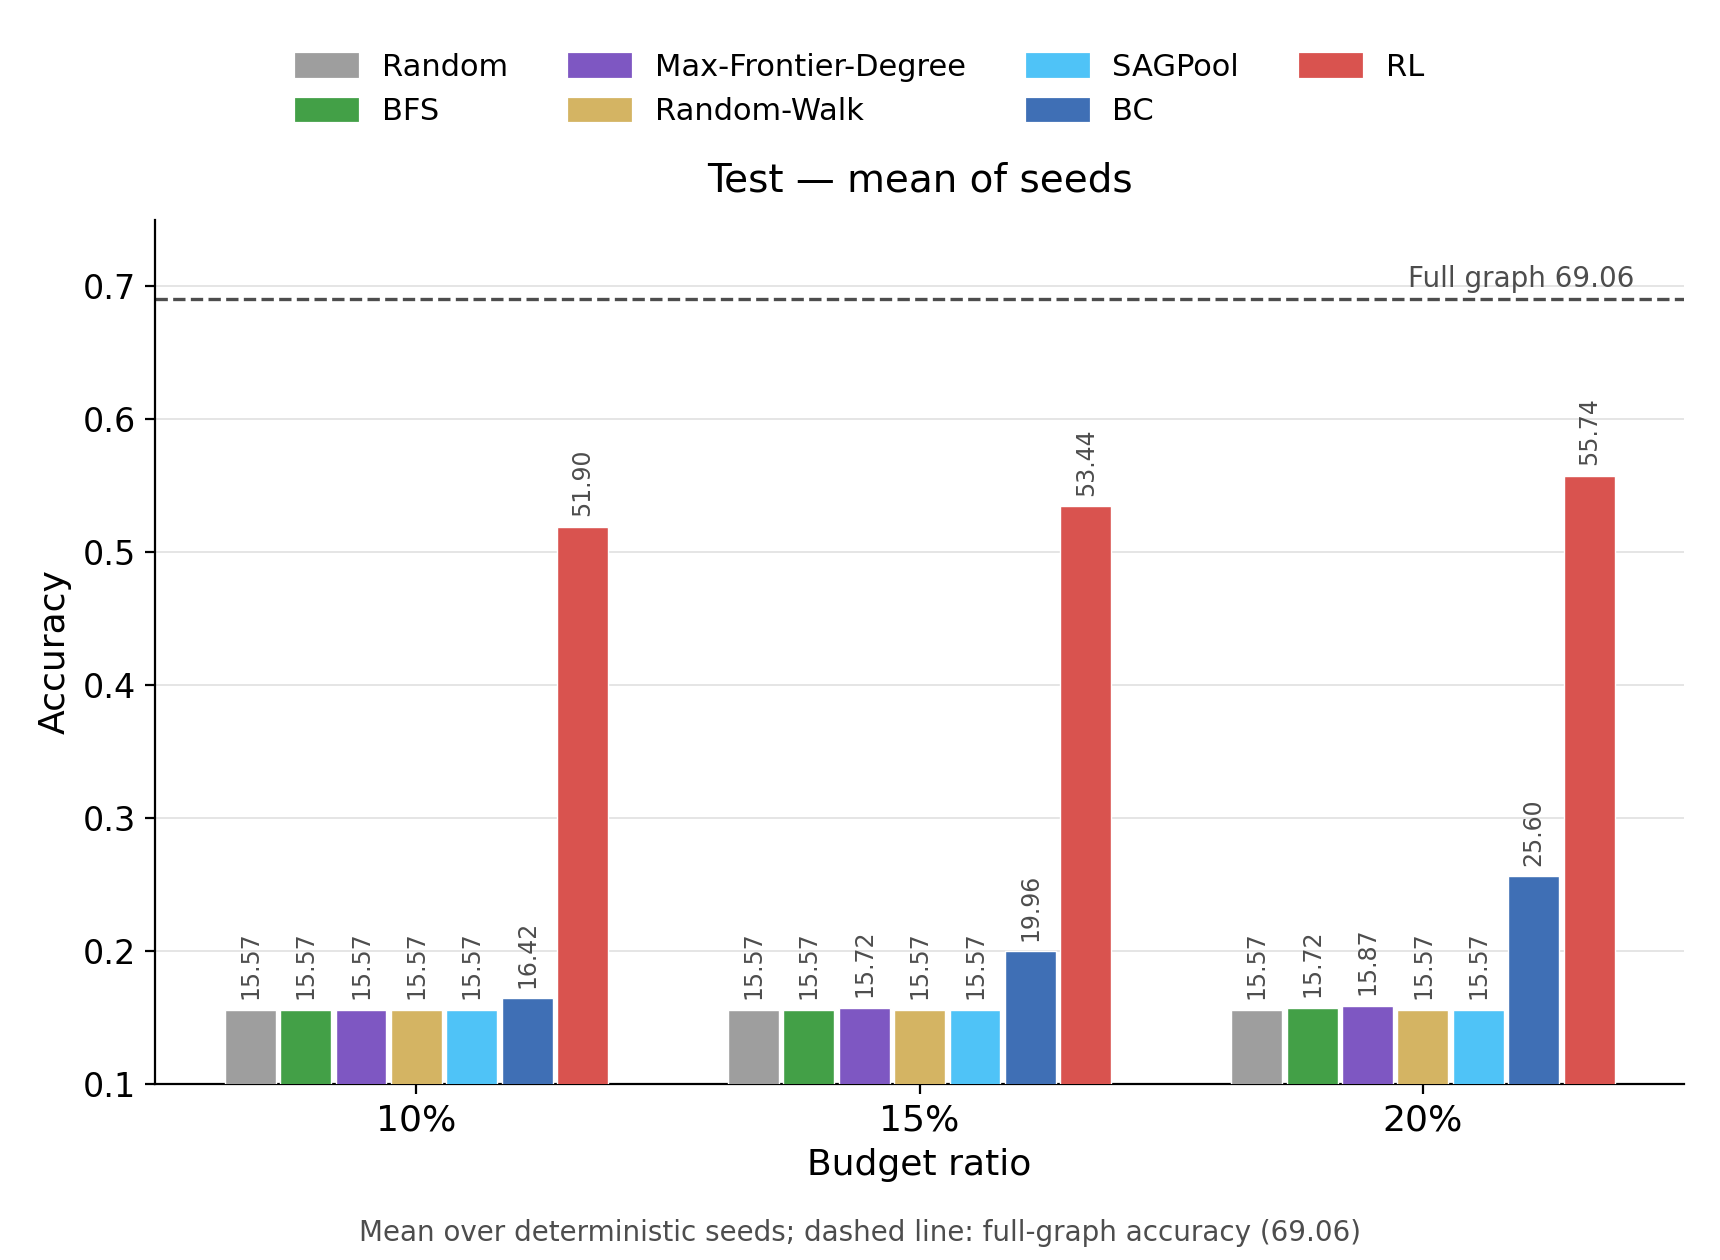
\includegraphics[width=0.92\linewidth]{figures/three_stage_compare_test.png}
\caption{COLLAB test accuracy under matched budgets (mean of 4 seeds). Fixed strategies and SAGPool stay at the majority-class rate ($\approx 0.16$); behavior cloning improves modestly; reinforcement fine-tuning reaches $0.52$--$0.56$ against the full-graph upper bound of $0.655$ (dashed).}
\label{fig:threestage}
\end{figure}

\subsection{Learned reading outperforms fixed strategies}
\label{sec:main-results}

On CIFAR10 superpixels (Table~\ref{tab:cifar10}, Figure~\ref{fig:cifar10-threestage}), fixed strategies cluster between $16$ and $21$ points, and behavior cloning sits within that band: imitating task-agnostic teachers does not by itself beat the best heuristic. Reinforcement fine-tuning moves the policy far outside the band, to $25.32$ at $5\%$, $30.03$ at $10\%$, and $32.68$ at $15\%$ budget, which is $+9.0$ to $+11.3$ points over the best fixed strategy at each budget and up to $+14.3$ points over BC. The gap between RL and the reference head ($32.68$ vs.\ $22.98$ at $15\%$) indicates that the learned policy reveals subgraphs that the frozen classifier reads \emph{better} than typical same-size subgraphs, rather than merely revealing more.

\begin{figure}[t]
\centering
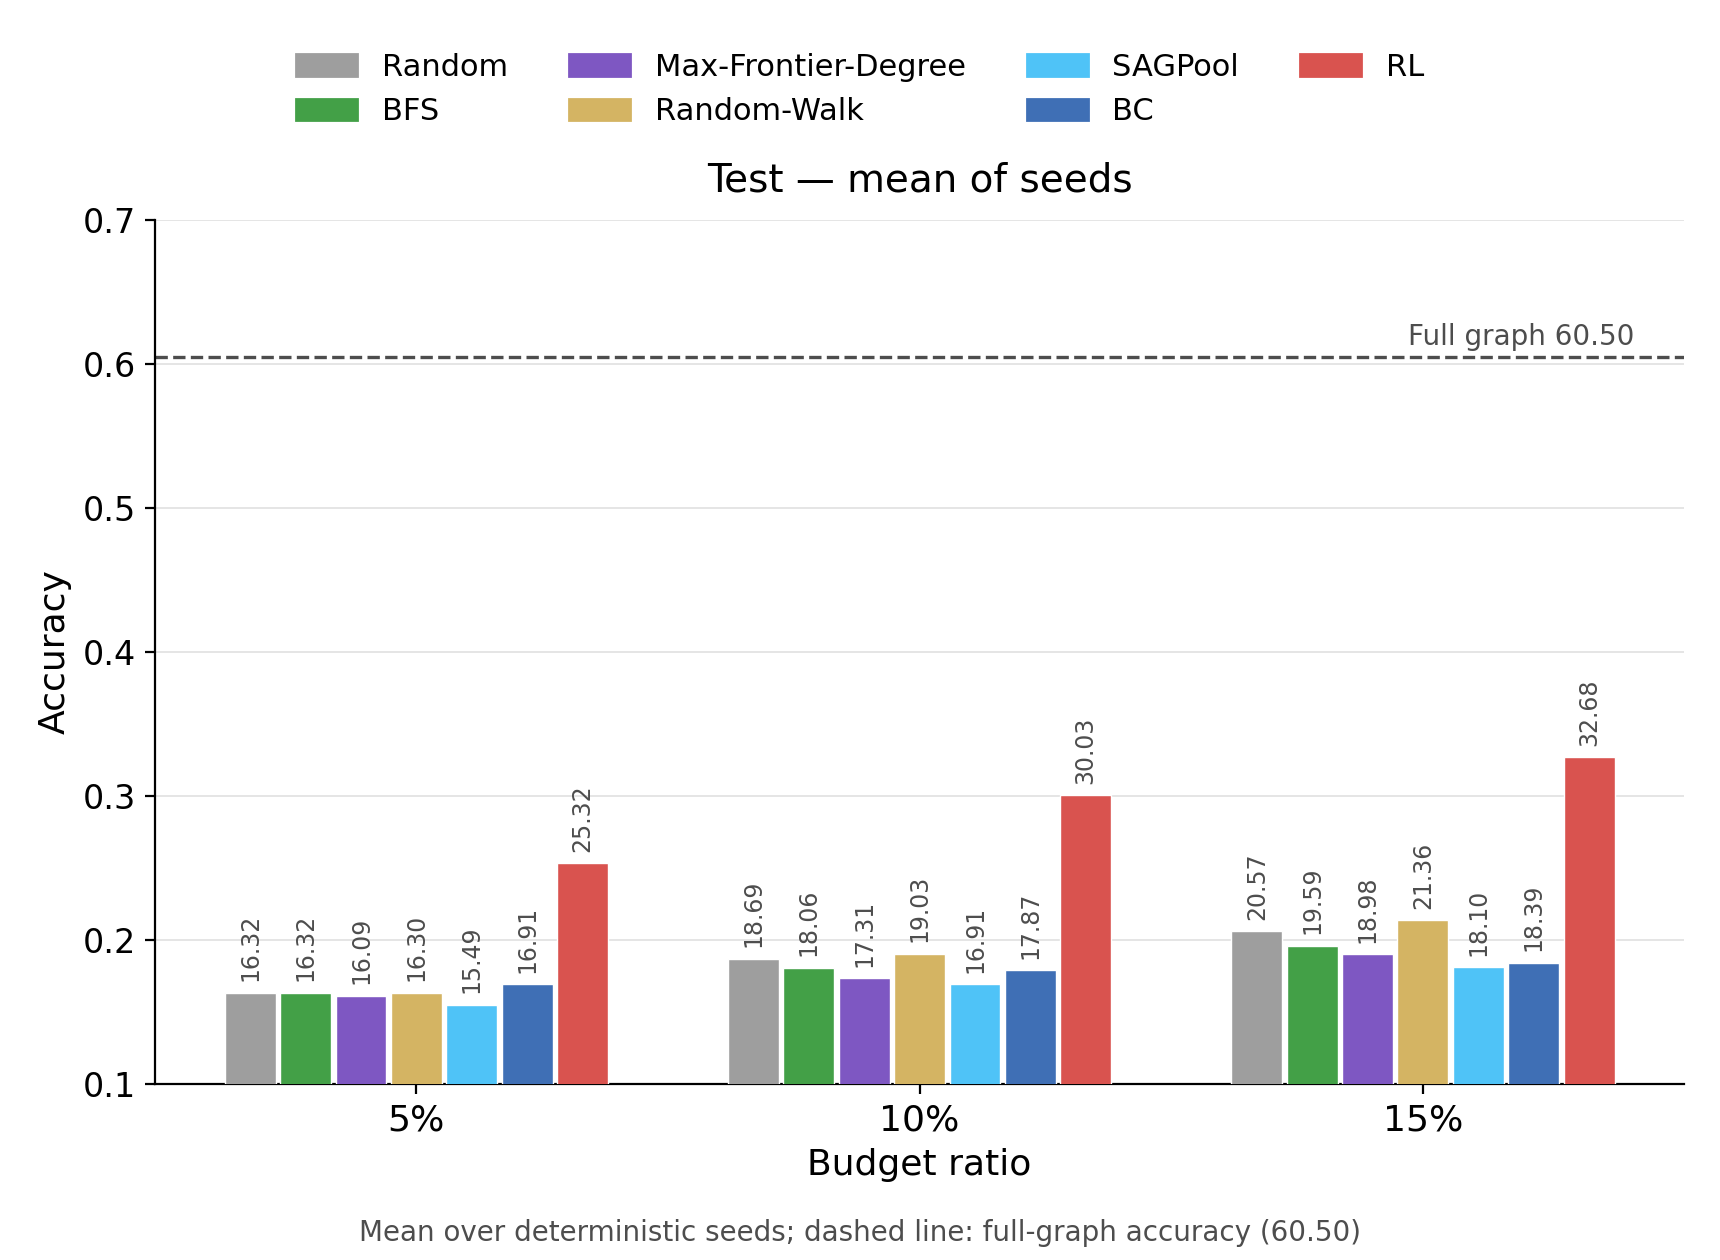
\includegraphics[width=0.92\linewidth]{figures/cifar10_three_stage_compare_test.png}
\caption{CIFAR10 superpixels, test accuracy under matched budgets (mean of 4 seeds). Behavior cloning stays within the fixed-strategy band, while reinforcement fine-tuning reaches $0.25$--$0.33$ against the full-graph upper bound of $0.605$ (dashed).}
\label{fig:cifar10-threestage}
\end{figure}

On COLLAB (Table~\ref{tab:collab}, Figure~\ref{fig:threestage}), every fixed strategy and SAGPool stays within $15.4$--$16.0$ on both splits, the majority-class rate of this imbalanced dataset: at $10$--$20\%$ budgets, task-agnostic selection never escapes the collapse. Behavior cloning improves to $16.8$--$27.6$ on validation and $16.4$--$25.6$ on test, and reinforcement fine-tuning reaches $51.90$, $53.44$, and $55.74$ on test, recovering $79\%$ to $85\%$ of the full-graph test accuracy ($65.5$). The reference head sharpens the contrast: the frozen classifier itself reads the RL-revealed subgraphs at only $15.7$--$20.3$, so the evidence head, not the frozen readout, is what converts revealed evidence into the prediction. The three-stage pattern in Figure~\ref{fig:threestage} repeats across datasets: fixed strategies bound what task-agnostic reading can do, BC makes a modest task-aware step, and RL supplies most of the gain.

\begin{table}[t]
\centering
\caption{OGBG-PPA, accuracy (\%), mean of 4 seeds. All cells report validation\,/\,test. On PPA the learned policies do not yet surpass the best fixed strategy (Section~\ref{sec:limitations}); BC collapses to near chance.}
\label{tab:ppa}
\footnotesize
\setlength{\tabcolsep}{2.5pt}
\begin{tabular}{lccccccc}
\toprule
Budget & Random & BFS & Max-Front.-Deg. & Rand.-Walk & SAGPool & BC & RL \\
\midrule
$5\%$  & 18.86\,/\,20.16 & 23.45\,/\,24.45 & 25.31\,/\,26.20 & 19.71\,/\,21.46 & 26.08\,/\,27.28 & 3.90\,/\,3.97 & 23.53\,/\,26.90 \\
$10\%$ & 31.14\,/\,33.07 & 30.06\,/\,35.68 & 36.33\,/\,37.28 & 32.34\,/\,34.54 & 36.25\,/\,37.92 & 7.23\,/\,7.37 & 28.12\,/\,32.34 \\
$15\%$ & 39.37\,/\,41.88 & 40.84\,/\,42.92 & 42.94\,/\,44.52 & 40.21\,/\,42.99 & 43.03\,/\,45.08 & 9.04\,/\,9.03 & 30.76\,/\,35.05 \\
\midrule
\multicolumn{8}{l}{\footnotesize Full-graph classifier (upper bound): 64.2 valid / 65.6 test.}
\\
\bottomrule
\end{tabular}
\end{table}

On OGBG-PPA (Table~\ref{tab:ppa}), fixed strategies separate cleanly and scale with budget, and SAGPool is the strongest fixed baseline on the test split. The learned policies do not currently compete on this dataset: behavior cloning collapses to $3.9$--$9.0$, far below every fixed strategy, and reinforcement fine-tuning, while consistently above its reference head ($20.7$--$33.0$), trails the best fixed baseline at every budget. We therefore make no adaptive-reading claim on PPA and return to this result in Section~\ref{sec:limitations}.

\subsection{Ablations}
\label{sec:ablation}

\begin{table}[t]
\centering
\caption{Behavior-cloning ablations, test accuracy (\%), mean of 4 seeds. ``no-pool'' removes attention pooling over read evidence; ``no-lstm'' removes the recurrent accumulator; ``v1'' removes both. COLLAB uses $10/15/20\%$ budgets.}
\label{tab:ablation}
\small
\begin{tabular}{llcccc}
\toprule
Dataset & Variant & \multicolumn{4}{c}{Budget levels} \\
\midrule
\multirow{4}{*}{CIFAR10}
 & full      & 18.35 & 20.07 & 20.45 & \\
 & no-pool   & 17.16 & 18.09 & 19.01 & \\
 & no-lstm   & 17.56 & 18.26 & 19.15 & \\
 & v1        & 16.91 & 18.58 & 19.38 & \\
\midrule
\multirow{4}{*}{COLLAB}
 & full      & 16.42 & 19.96 & 25.60 & \\
 & no-pool   & 15.72 & 18.41 & 21.11 & \\
 & no-lstm   & 15.72 & 18.21 & 20.11 & \\
 & v1        & 15.88 & 18.04 & 20.64 & \\
\bottomrule
\end{tabular}
\end{table}

Table~\ref{tab:ablation} and Figure~\ref{fig:ablation} isolate the two components of the evidence reader. Recurrent accumulation is the largest contributor on COLLAB: removing the LSTM costs $5.5$ points at the $20\%$ budget ($25.60 \to 20.11$), and removing both components costs $5.0$ points while degrading most at the largest budget. On CIFAR10 the effects are smaller but consistent, with attention pooling contributing $1.0$--$1.4$ points and the full variant leading at every budget. The pattern matches the design rationale: long-range evidence integration matters most on sparse, long-diameter graphs such as COLLAB, where revealed subgraphs stay connected but their diameter exceeds the encoder's reach.

\begin{figure}[t]
\centering
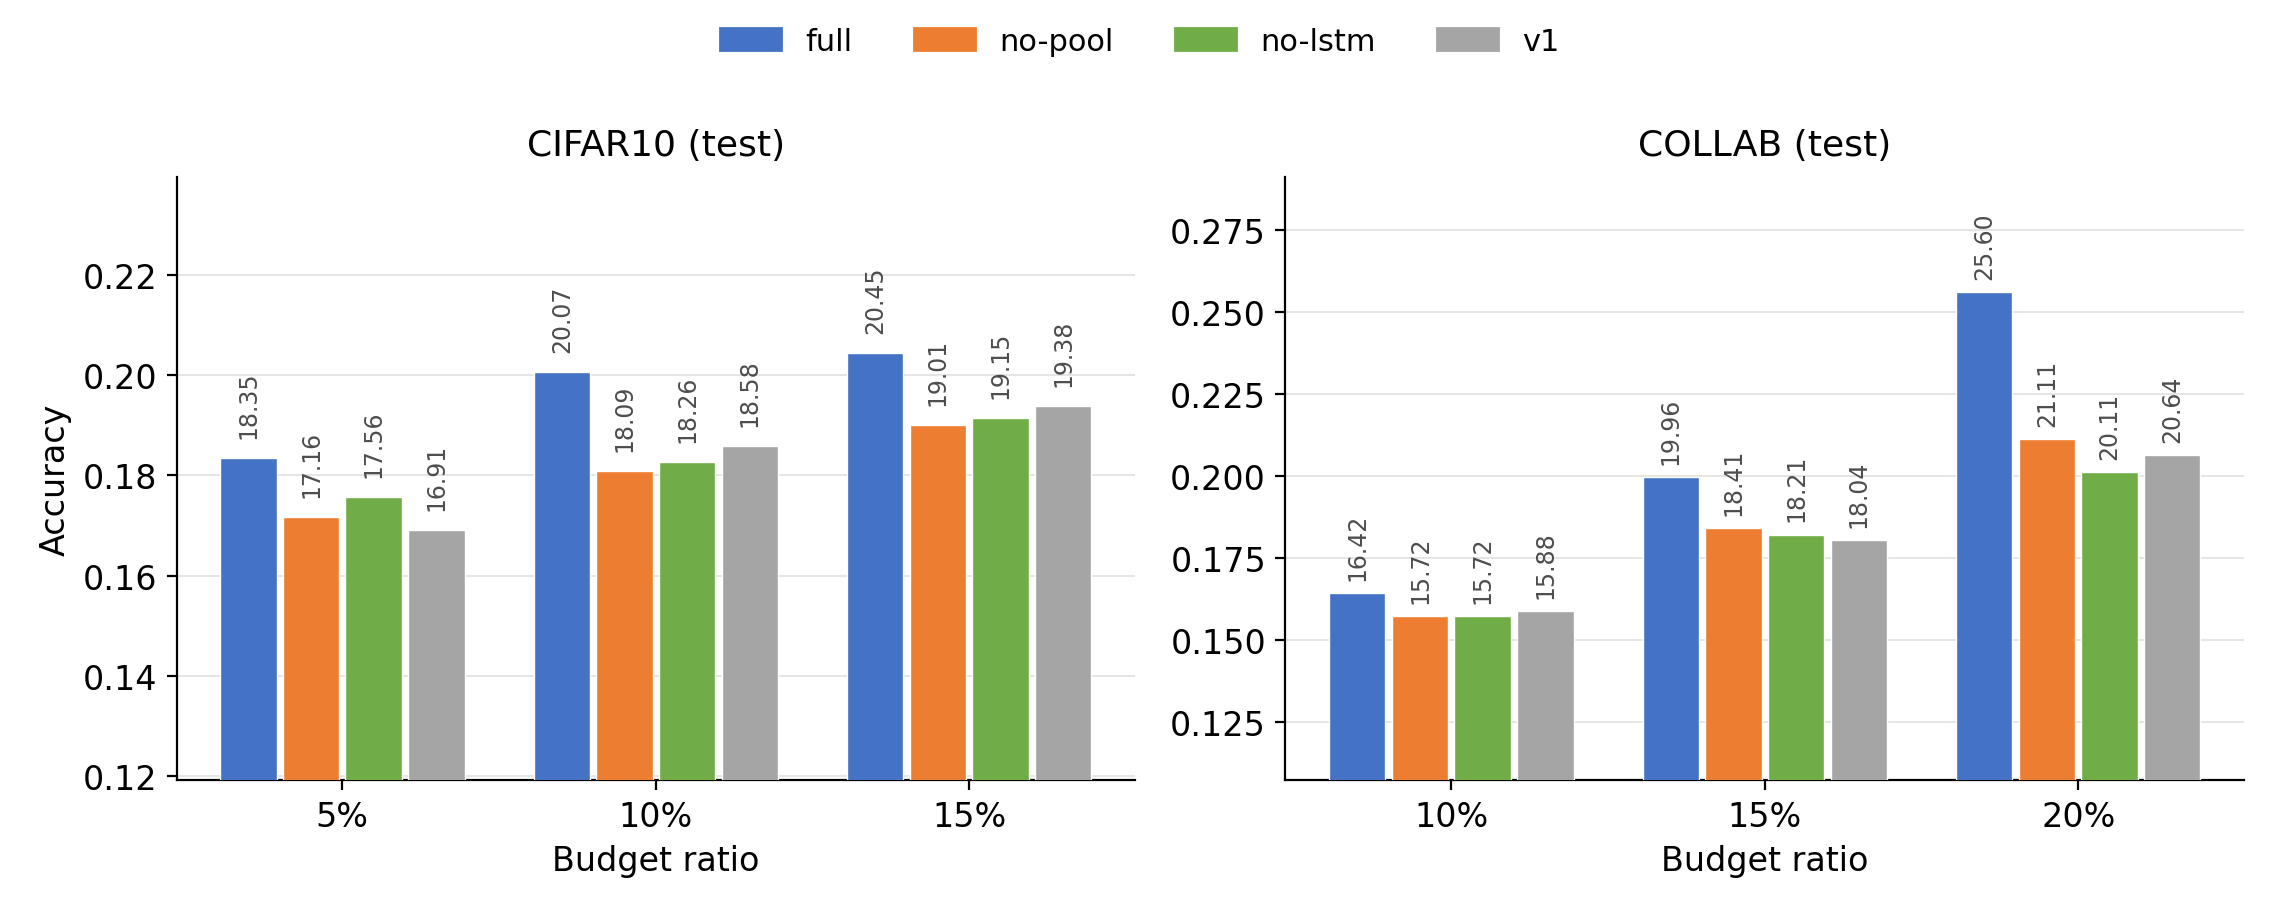
\includegraphics[width=0.98\linewidth]{figures/bc_ablation.png}
\caption{Behavior-cloning ablations on the test split (mean of 4 seeds). Left: CIFAR10 superpixels at $5/10/15\%$ budgets. Right: COLLAB at $10/15/20\%$ budgets. Removing the recurrent accumulator (no-lstm) or both components (v1) hurts most on COLLAB, where revealed subgraphs have long diameters.}
\label{fig:ablation}
\end{figure}

\section{Discussion and limitations}
\label{sec:limitations}

\paragraph{What the gains mean.}
Two mechanisms contribute to the RL gains, and the reference head helps separate them. Part of the gain is selection: the policy finds informative regions. Part is calibration: repeated reveal patterns may better match how the frozen classifier was trained on full graphs. Because RL's final predictions beat the same classifier's accuracy on typical revealed subgraphs by a wide margin on CIFAR10, selection appears to be the dominant mechanism, but we cannot fully exclude calibration effects without a matched-training control, which we leave to future work.

\paragraph{Boundaries of the current evidence.}
First, gains shrink at the smallest budgets: at $5\%$ of CIFAR10, RL recovers well under half of the full-graph accuracy, so the approach currently suits regimes where a moderate fraction of nodes can be inspected. Second, accuracy is uneven across classes: on CIFAR10, the hardest classes remain near chance on test with a $71.7$-point spread between best and worst classes, indicating a capability boundary rather than a data-quantity problem, since class-balanced filtering changed little. Third, OGBG-PPA is a negative result for the current method: behavior cloning collapses to near chance, and RL, though consistently above its reference head, does not surpass the best fixed strategy at any budget; whether this reflects reward sparsity, the budget granularity of PPA graphs, or class imbalance is open, and we draw no adaptive-reading conclusion from it. Fourth, the protocol assumes single-label, mutually exclusive classification; multi-label and regression targets require changes to the reward and metrics that the current implementation does not support.

\section{Conclusion}
\label{sec:conclusion}

We formalized budget-limited active graph reading with a leak-proof protocol, and showed that a two-stage learner, behavior cloning followed by reinforcement fine-tuning with an asymmetric reward, turns task-agnostic reading into task-aware reading: on COLLAB it recovers up to $85\%$ of full-graph test accuracy with $20\%$ of nodes revealed, where all fixed strategies collapse to the majority-class rate, and on CIFAR10 it outperforms the best fixed strategy by up to $11.3$ points. Recurrent evidence accumulation, decoupled from node selection, carries the largest share of the improvement. The results bound themselves: gains narrow at very small budgets, hard classes remain unsolved, and on PPA the learned policy does not yet beat the best fixed strategy; closing these gaps, together with a calibration-controlled attribution of the gains, is the next step toward reading large graphs the way agents read long documents: selectively, and on a budget.

\subsubsection*{Reproducibility statement}
All experiments use deterministic seed formulas per graph and budget, fixed split definitions, and a single evaluation schema with per-class breakdowns; configs are embedded in every checkpoint and results are reported as means over four seeds. Code, configurations, trajectory data, and the leakage-invariant test suite will be released upon publication. Training details, teacher construction, the reward family ablation, and per-class diagnostics are provided in the supplement.

\subsubsection*{LLM usage statement}
An LLM-based coding assistant was used for implementing the experimental codebase and for drafting support; all results, claims, and conclusions were produced and verified by the authors, who take full responsibility for the content. (Per ICLR policy, this statement will be moved to the appendix in the submitted version.)

\end{document}
